\documentclass[10pt, a5paper]{article}
\usepackage{pdfpages}
\usepackage{parallel}
\usepackage[T2A]{fontenc}
\usepackage{ucs}
\usepackage[utf8x]{inputenc}
\usepackage[polish,english,russian]{babel}
\usepackage{hyperref}
\usepackage{rotating}
\usepackage[inner=2cm,top=1.8cm,outer=2cm,bottom=2.3cm,nohead]{geometry}
\usepackage{listings}
\usepackage{graphicx}
\usepackage{wrapfig}
\usepackage{longtable}
\usepackage{indentfirst}
\usepackage{array}
\newcolumntype{P}[1]{>{\raggedright\arraybackslash}p{#1}}
\frenchspacing
\usepackage{fixltx2e} %text sub- and superscripts
\usepackage{icomma} % коскі ў матэматычным рэжыме
\PreloadUnicodePage{4}

\newcommand{\longpage}{\enlargethispage{\baselineskip}}
\newcommand{\shortpage}{\enlargethispage{-\baselineskip}}

\def\switchlang#1{\expandafter\csname switchlang#1\endcsname}
\def\switchlangbe{
\let\saverefname=\refname%
\def\refname{Літаратура}%
\def\figurename{Іл.}%
}
\def\switchlangen{
\let\saverefname=\refname%
\def\refname{References}%
\def\figurename{Fig.}%
}
\def\switchlangru{
\let\saverefname=\refname%
\let\savefigurename=\figurename%
\def\refname{Литература}%
\def\figurename{Рис.}%
}

\hyphenation{admi-ni-stra-tive}
\hyphenation{ex-pe-ri-ence}
\hyphenation{fle-xi-bi-li-ty}
\hyphenation{Py-thon}
\hyphenation{ma-the-ma-ti-cal}
\hyphenation{re-ported}
\hyphenation{imp-le-menta-tions}
\hyphenation{pro-vides}
\hyphenation{en-gi-neering}
\hyphenation{com-pa-ti-bi-li-ty}
\hyphenation{im-pos-sible}
\hyphenation{desk-top}
\hyphenation{elec-tro-nic}
\hyphenation{com-pa-ny}
\hyphenation{de-ve-lop-ment}
\hyphenation{de-ve-loping}
\hyphenation{de-ve-lop}
\hyphenation{da-ta-ba-se}
\hyphenation{plat-forms}
\hyphenation{or-ga-ni-za-tion}
\hyphenation{pro-gramming}
\hyphenation{in-stru-ments}
\hyphenation{Li-nux}
\hyphenation{sour-ce}
\hyphenation{en-vi-ron-ment}
\hyphenation{Te-le-pathy}
\hyphenation{Li-nux-ov-ka}
\hyphenation{Open-BSD}
\hyphenation{Free-BSD}
\hyphenation{men-ti-on-ed}
\hyphenation{app-li-ca-tion}

\def\progref!#1!{\texttt{#1}}
\renewcommand{\arraystretch}{2} %Іначай формулы ў матрыцы зліпаюцца з лініямі
\usepackage{array}

\def\interview #1 (#2), #3, #4, #5\par{

\section[#1, #3, #4]{#1 -- #3, #4}
\def\qname{LVEE}
\def\aname{#1}
\def\q ##1\par{{\noindent \bf \qname: ##1 }\par}
\def\a{{\noindent \bf \aname: } \def\qname{L}\def\aname{#2}}
}

\def\interview* #1 (#2), #3, #4, #5\par{

\section*{#1\\{\small\rm #3, #4. #5}}

\def\qname{LVEE}
\def\aname{#1}
\def\q ##1\par{{\noindent \bf \qname: ##1 }\par}
\def\a{{\noindent \bf \aname: } \def\qname{L}\def\aname{#2}}
}


\begin{document}

\title{Linux и СПО в создании музыки и живом исполнении. Обзор имеющихся программ и ниши применения}
\author{Сергей Васильев\footnote{Таллинн, Эстония, \url{zyxos2@gmail.com}}}
\date{}
\maketitle
\begin{abstract}
The aspects of using Linuz and free software in amateur music creation, sound editing and live performances are reviewed.
\end{abstract}

Ещё несколько лет назад Linux был малопригоден для работы со звуком; за последние годы ситуация значительно изменилась: улучшилась поддержка многих звуковых карт, MIDI-контроллеров и MIDI-интерфейсов, появились новые программы, интерфейс которых изменился в лучшую сторону, что снизило порог вхождения для начинающих пользоваталей. И, несмотря на некоторые всё ещё присутствующие проблемы, сейчас вполне возможно использование решений на базе Linux и СПО в любительской музыкальной деятельности. Применение данных решений имеет ряд преимуществ, одним из которых является низкая стоимость, что немаловажно для начинающих музыкантов. 

Многие начинающие музыканты не обращают внимания на Linux из-за недостаточной информированности, и очень часто для выполнения простых задач прибегают к применению программного обеспечения, возможности которого на порядок превышают потребности, что приводит к нерациональному расходу денежных средств или к незаконному использованию коммерческих приложений. Имеющейся на данный момент программной базы и поддержки оборудования достаточно для выполнения основных задач. 

В таблице приведены категории и некоторые программы, которые, после сравнительного анализа, были отобраны как наиболее подходящие для использования в сетапе для демонстрации.

\begin{figure}[ht]
\centering{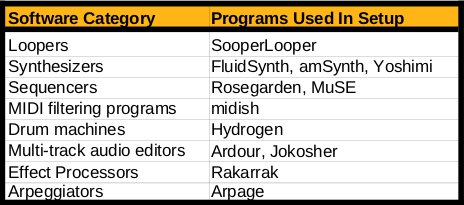
\includegraphics[width=8cm]{13_abstract.jpg}}
%\label{pic:fl1}
\caption{Приложения по категориям}
\end{figure}

По субъективной оценке, наиболее заполнены категории многодорожечных аудиоредакторов, представленных мощнейшим проектом Ardour, и некоторыми более простыми; процессоров эффектов --- Rakarrak и др.; также почти на 100\% покрывает потребности замечательный редактор табулатур TuxGuitar.

Драм-машины представлены практически одним проектом Hydrogen, но довольно мощным, лишь с небольшими пожеланиями усовершенствований в области мульти-лэйеринга.

Что касается луперов и арпеджиаторов --- лидеры SooperLooper и Arpage предоставляют базовую функциональность, но хотелось бы надеяться на улучшения в будущем.

Категории с некоторым количеством недочетов --- секвенсеры и MIDI-фильтры.

Проблемные категории --- синтезаторы (несмотря на замечательные программы FluidSynth, amSynth и Yoshimi, ситуация  c VST-плагинами все еще далека от идеальной) и автоаккомпаниаторы (поскольку MMA очень сильно нехватает адекватного GUI).
\end{document}
